\begin{frame}[label=intro]
    \frametitle{¿Qué es Prometheus?}
    \begin{columns}
        \begin{column}{0.6\textwidth}
            \begin{figure}[H]
                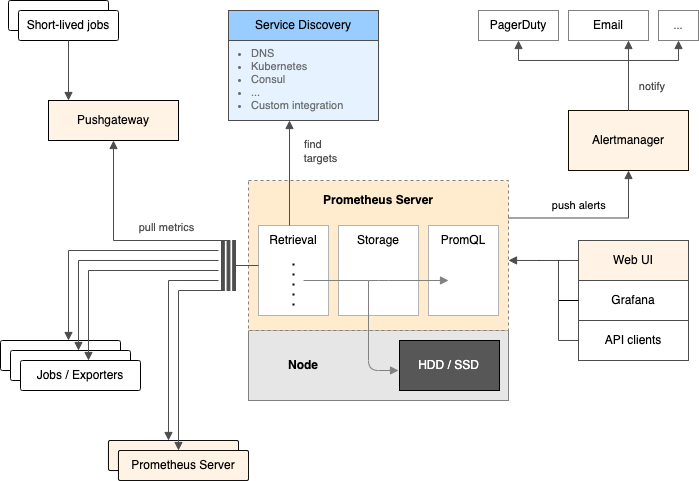
\includegraphics[width=\textwidth]{include/prometheus_arch.png}
                \caption{Arquitectura de funcionamiento de Prometheus}
            \end{figure}
        \end{column}
        \begin{column}{0.45\textwidth}
            \centering
            ¿Qué se necesita para monitorizar con Prometheus?
            \begin{itemize}
                \item Servidor de prometheus
                \item Targets con etiquetas,\\ agrupados por proyectos
                \item Reglas de alertado
            \end{itemize}
        \end{column}
    \end{columns}
    \input{secciones/notas/intro_prometheus_notes}
\end{frame}